\section{Il bilancio di esercizio}
\subsection{Circolare capitale netto}
Rappresenta la quota di capitale di esercizio finanziaria con risorse a disposizione dell'azienda in via stabile e permanente.

Rappresentata da differenza tra attività a breve e passività a breve.

\subsection{Margine di tesoreria}
(Attività correnti - magazzino netto) - Passività correnti

Capacità dell'impresa di fare fronte a cose con solo le liquidità immediate.

\subsection{Margine di struttura}
Capitale netto - immobilizzazione nette

\subsection{Indici di bilancio}
La liquidità di un'azienda è data dalla sua capacità di onorare le obbligazioni che scadono nel breve(solvibilità a breve).

\begin{equation*}
    \text{Indice di liquidità corrente o disponibilità} = \frac{\text{Attivo corrente}}{\text{Passivo corrente}}
\end{equation*}

\begin{itemize}
    \item $\geq 1,5$ equilibrio
    \item $> 1, < 1,5$ attenzione
    \item $< 1$ squilibrio
\end{itemize}

\subsection{Indice Indice di liquidità immediata}
\begin{equation*}
    \text{Indice di liquidità immediata} = \frac{\text{Attivo corrente} - \text{Rimanenze}}{\text{Passivo corrente}}
\end{equation*}

\begin{itemize}
    \item tra 0,5 e 1 situazione di equilibrio
    \item tra 0,33 e 0,5 attenzione
    \item se sotto 0,33 situazione di squilbrio
\end{itemize}

\subsection{Indici di solidità patrimoniale}
Permettono di capire la solvibilità a medio lungo termine.

\subsubsection{Tasso di indebitamento Leverage(D/E)}
\begin{equation*}
    \text{D/E} = \frac{\text{Mezzi di terzi}}{\text{Patrimonio netto}} \leq 1
\end{equation*}

\subsubsection{Indice di autocopertura delle immobilizzazioni}
Il patrimonio netto copre le immobilizzazioni
\begin{equation*}
    \text{Indice di autocopertura delle immobilizzazioni} = \frac{\text{Patrimonio netto}}{\text{Immobilizzazione}}
\end{equation*}

\begin{itemize}
    \item $\geq 0,7$ equilibrio
    \item $< 0,7$ attenzione
    \item $< 0,5$ squilibrio
\end{itemize}

\subsubsection{Indice di copertura delle immobilizzazioni}
Gli investimenti sono coperti delle fonti finanziarie a lungo termine.

\begin{equation*}
    \text{Indice di copertura delle immobilizzazioni} = 
    \frac{
        \text{Debiti a m/l termine} + \text{Patrimonio netto}
    }{
        \text{Immobilizzazioni}
    }
\end{equation*}

\begin{itemize}
    \item $\geq 1,5$ equilibrio
    \item $< 1,5$ attenzione
    \item $< 1$ squilibrio
\end{itemize}

\subsubsection{Indice di indipendenza finanziaria(IIF)}
\begin{equation*}
    \text{IIF} = \frac{\text{Patrimonio netto}}{\text{Attivo netto}}
\end{equation*}

\begin{itemize}
    \item 1 ideale
    \item tra 0,5 e 0,75 equilibrio
    \item sotto 0,5 squilibrio
\end{itemize}

\subsection{Indici di redditività}
Capacità di produrre utile attraverso lo svolgimentodell'impresa.

\subsubsection{ROE(return of equity)}
\begin{equation*}
    \text{ROE \%} = \frac{\text{Reddito netto}}{\text{Patrimonio netto}}
\end{equation*}

\subsubsection{IDEO - Incidenza gestione extra-operativa}
\begin{equation*}
    \text{IGEO} = \frac{\text{Reddito netto}}{\text{Risultato operativo (EBIT) Aziendale}}
\end{equation*}

\subsubsection{ROA - return on net asset}
\begin{figure}[H]
    \centering
    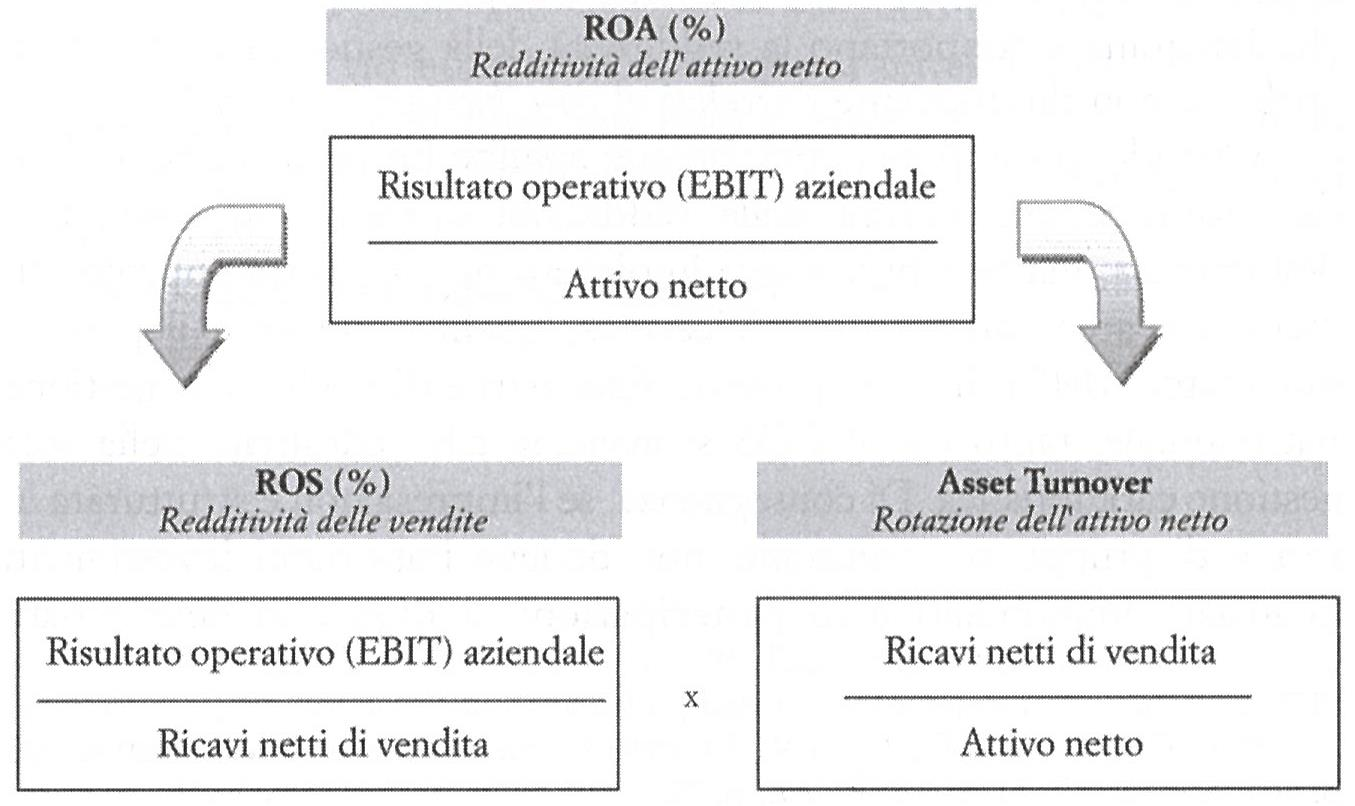
\includegraphics[width=0.7\linewidth]{2/img/ROA.png}
\end{figure}
\begin{equation*}
    \text{ROA \%} = \frac{\text{Risultato operativo (EBIT) aziendale}}{Attivo netto}
\end{equation*}

\subsubsection{Asset turnover}
Indica l'intensità con la quale l'azienda sfrutta i sui investimenti in attività operative.

\begin{equation*}
    \text{Asset Turnover} = \frac{\text{Ricavi netti}}{\text{Attivo netto}}
\end{equation*}

\subsubsection{ROS - Retunr on sales}
\begin{equation*}
    \text{ROS \%} = \frac{
        \text{
            Risultato operativo (EBIT) aziendale
        }
    }{
        \text{
            Ricavi netti
        }
    }
\end{equation*}

\subsubsection{ROD - return on debit}

\begin{equation*}
    \text{ROD \%} = \frac{
        \text{
            Oneri finanziari
        }
    }{
        \text{
            Mezzi di terzi
        }
    }
\end{equation*}

\subsubsection{Tasso di incidenza della gestione fiscale (t)}
\begin{equation*}
    t = \frac{
        \text{
            imposte sul reddito
        }
    }{
        \text{
            risultato ante imposte
        }
    }
\end{equation*}

\begin{equation*}
    \text{
        reddito netto
    } = \text{
        risultato ante imposte 
    }
    (1 - t)
\end{equation*}

\subsubsection{Leva finanziaria}
\begin{equation*}
    \text{ROE} = \frac{
        \text{
            RN
        }
    }{
        \text{
            RAI
        }
    } \Big[\text{ROA} + \Big(\text{ROA} - \text{ROD}\Big) \frac{\text{MT}}{\text{PN}}\Big]
\end{equation*}

\begin{itemize}
    \item \textbf{RN/RAI}: risutlato netto fratto risultato ante imposte
    \item \textbf{ROA}: Indice return on asset
    \item \textbf{MT}: debiti di finanziamento ad interesse esplicito
    \item \textbf{PN}: patrimonio netto
    \item \textbf{MT/MN}: indice di indebitamento (\textbf{D/E})
    \item \textbf{ROD}: oneri finanziari fratto debiti
\end{itemize}

Altre versione per scrivere questa cacata è quello di sostituire $\frac{\text{RN}}{\text{RAI}}$ con 
$(1 - t)$, si ottiene:
\begin{equation*}
    \text{ROE} = 
    \Big[\text{ROA} + \Big(\text{ROA} - \text{ROD}\Big) \frac{\text{MT}}{\text{PN}}\Big] (1 - t)
\end{equation*}

\begin{itemize}
    \item \textbf{$t$}: tasso di incidenza della gestione fiscale
\end{itemize}

ROA è maggiore di ROA solo se ROA è maggiore di ROD, leffetto della leva risulta:
\begin{equation*}
    \text{ROA} - \text{ROD} > 0
\end{equation*}

Così si ottiene una leva positiva, ma se ROD è maggiore di ROA, si ottiene una leva negativa!!

